\documentclass[article,a4paper,oneside]{article}
%% Math stuffs
\usepackage[utf8]{inputenc}
\usepackage[english]{babel}
\usepackage[T1]{fontenc}
\usepackage{amssymb}
\usepackage{amsmath}
\usepackage{amsthm}
\usepackage{todonotes}
\usepackage{hyperref}
\usepackage{graphicx}
\newtheorem{thm}{Theorem}

%%We have quite a bit of math inline, so let's remove the paragraph indent and instead move it a bit down
\parindent 0pt
\parskip 4mm
%% for easy Matrix notation
\newcommand{\+}[1]{\ensuremath{\boldsymbol{#1}}}

%%For syntaxhighligting when needed:
%%remember to invoke pdflatex with -shell-escape when not commented out
\usepackage{minted}

\begin{document}
\title{
Randomized Algorithms Project 1\\
Analysis and experiments with randomized kth find and randomized quicksort
}

\author{
  Mads Ravn - 20071580\\
  Bo Mortensen - 20073241\\
  Johan Abildskov - 20063623
}

\date{\today}

\maketitle

\newpage


\subsubsection*{Introduction}
In the following report we will prove a bound on finding the $k$th smallest as well as show experiments relating to the theoretical bounds. We will do a similar experimentation for \emph{randomized QuickSort}.

\subsection*{\texttt{FIND}}
In this section we look at the problem of finding the $k$th smallest integer in a list $L$. That is, given an unsorted list $L$, return the $k$th smallest element.
The algorithm is given here:
\begin{center}\begin{minipage}{5in}
\underline{Algorithm: FIND}\\
\begin{tabular}{ll}
Input: & $L=[a_1,\ldots,a_n]$, a nonempty list of distinct numbers\\
& $k$, an integer such that $1\leq k\leq n$.\\ 
Output: & $b$, where $b\in L$ and $|\{a\in L:a\leq b\}|=k$\\
Method:\\
{\hfill}1. & Select $e$ randomly from $L$ using the uniform distribution\\
{\hfill}2. & Split $L'=L-\{e\}$ into the two sublists\\
& \ \ $L_1=[a_i\in L|a_i<e]$\\
& and\\
& \ \ $L_2=[a_i\in L|a_i>e]$\\
& by comparing $e$ to each element of $L'$.\\
{\hfill}3. & If $|L_1|=k-1$ then return $e$.\\
& If $|L_1|>k-1$ then make a recursive call on $L_1$ and $k$.\\
& \begin{minipage}{4in}
If $|L_1|<k-1$ then make a recursive call on $L_2$ and $k-1-|L_1|$.
\end{minipage}
\end{tabular}
\end{minipage}\end{center}
As we can see the approach is quite similar to that of a randomized quicksort.
We are following the suggested approach from the project description.
\par

Let $\pi$ be the unique permutation that sorts the elements of $L$,
i.e. $a_{\pi(1)}<\cdots <a_{\pi(n)}$.  Define the indicator variables

$$Z_{i}=\left\{\begin{array}{ll}
1, & \mbox{
\begin{minipage}[t]{4in}
  if $a_{\pi(i)}$ is selected as the random element $e$ in line 1
  during any of the recursive executions of FIND
\end{minipage}
}
\\
0, & \mbox{ otherwise}
\end{array}\right.$$

Define:

$$Z=\sum_{i\neq k} Z_i$$

{\bf 1.1 \ Subproblem} Argue that $1+Z$ denotes the recursion depth
during the FIND execution.

Each index in $Z_i$ that is set to $1$ as defined above represents an added layer in the recursion, as this represents that the element at some point was chosen as the pivot element around which we create the two lists, one of which we will recurse in. The additional $1$ comes from the fact that we have defined $Z$ as the sum of indicator variables, except for $i=k$. This element itself obviously represents the point at which we have chosen the $k$th element as our pivot, and this adds the last layer of our recursion.
\par

{\bf 1.2 \ Subproblem} Prove that $$\Pr(Z_{i}=1)=\frac{1}{|k-i|+1}$$.

Consider that permutation $\pi$ as described above. We will look at the probability that any $a_{\pi(i)}$ is selected in the execution of \texttt{FIND}. Without loss of generality we look only at $\pi(i) < \pi(k)$. Consider now the subset of elements $$S = \lbrace a_{\pi(i)},\cdots,a_{\pi(k)}\rbrace$$ it is seen that the element $a_{\pi(i)}$ will be chosen as a pivot element \emph{iff} it is the \emph{first} element of $S$ to be chosen. If another element is chosen from $S$ then $a_{\pi(i)}$ will end up in the list that the algorithm does not do recursive work in. As each element in $S$ is equally likely to be chosen and the size of $S$ is $|k - i| + 1$, the probability that $i$ will be chosen first is $\frac{1}{|k-i |+1}$. We have thus proved that $$Pr[Z_{i} = 1] = \frac{1}{|k-i|+1}$$

{\bf 1.3 \ Subproblem} Prove that $E[Z]\leq \mu = 2 \ln n$.

For any $k, 0<k<n$ we have that $Z = \sum_{i=1}^{n} \frac{1}{|k-i|+1}$.
This gives cause to the following:

\begin{align*}
E[Z] &= \sum_{i=1}^{n} \frac{1}{|k-i|+1}
\\ &\leq \sum_{i=1}^{k-1} \frac{1}{i} + \sum_{i=k+1}^{n} \frac{1}{i}
\\ &\leq \sum_{i=1}^{k-1} \frac{1}{i} + \sum_{i=1}^{k-1} \frac{1}{i}
\\ &= 2\sum_{i=1}^{k-1} \frac{1}{i+1}
\\ &\leq 2H_n
\\ &\approx 2lnn \qedhere
\end{align*}

{\bf 1.4 \ Subproblem} Argue that $Z_1,Z_2,\ldots,Z_{k-1}$ are independent 
(and, similarly, $Z_{k+1},Z_{k+2},\ldots,Z_n$  are independent)

To show that $Z_i$ and $Z_j$ are independent for $i,j < k$, consider the case $Z_i = 1$. This means that in the interval $\mathbb{I} = [Z_i,..,Z_k]$, $Z_i$ was the first to be chosen as the random pivot element.
For any $Z_j, j \neq i$ we're considering the interval $\mathbb{J} = [Z_j,\ldots, Z_k]$, as $i \neq j \Rightarrow \mathbb{I} \neq \mathbb{J}$, we invoke the \emph{Principle of deferred decisions} and see that the two intervals are not related, and thus the choice of $Z_i$ and $Z_j$ is independent.

{\bf 1.5 \ Subproblem}
Prove that $\Pr(Z>2\mu)\leq 2 n^{-c}$ for as
large a constant $c$ as you can.

From (1.4) we have that $Z_1, Z_2, \ldots, Z_{k-1}$ are independent and $Z_{k+1}, Z_{k+2}, \ldots, Z_n$ are independent, and as such, the Chernoff bound technique can be applied in this situation. We denote the set of $Z_1, Z_2, \ldots, Z_{k-1}$ as $A$ and the set of $Z_{k+1}, Z_{k+2}, \ldots, Z_n$ as $B$. We know from (1.3) that the expected value of $A$ and $B$ are upper bounded by $\ln n$. We now utilize the Chernoff bound technique on the set $A$

$$\Pr \left( A > (1+\delta)\mu \right) < \left[ \frac{e^\delta}{(1+\delta)^{1+\delta}} \right]^\mu$$

\begin{align*}
  Pr( A > 2\mu) & <  \left[ \frac{e^1}{(1+1)^{1+1}} \right] ^{\ln n} \\
  &= \frac{e^{\ln n}}{4^{\ln n}}\\ 
  &= \frac {n}{e^{\ln(4)\ln(n)}} \\
  &= \frac{n}{n^{\ln(4)}}\\
  &= n^{1-\ln (4)}\\
\end{align*}

The exact same thing applies for $B$ and now we have $\Pr ( Z > 2\mu)$ expressed as $ \Pr ( A > 2\mu \vee B > 2\mu) = \Pr ( A > 2\mu) + \Pr( B > 2\mu) \leq 2n^{1-\ln(4)}$. We now have that $\Pr ( Z > 2\mu) \leq 2n^{1-\ln(4)}$ and thusly have a constant $\underline{c=\ln(4)-1}$.

{\bf 1.6 \ Subproblem} Implement the FIND algorithm and run it on a
representative set of test inputs. 
The algorithm \texttt{FIND} has been implemented in \texttt{C++11} and compiled with \texttt{clang} on a Linux machine with the optimization flag \texttt{-O3}.
\par
We have generated random lists of up to $10^5$ elements and have run the algorithm $10^6$ times  for each $k \in \lbrace 1, \frac{1}{10}n, \frac{2}{10}n, \ldots, n\rbrace$. The results can be seen in \ref{fig:qs}.
As can be seen from the table, the experimental results do not exceed the bounds given previously. The experimental results are indeed quite a bit below the bounds given. This could come from the fact that we introduce a lot of slack in the definition to obtain the nice looking bound, and it therefore is less tight.

\begin{center}
\begin{figure}
\caption{Results from running \texttt{FIND}}
\label{fig:qs}
\begin{tabular}{| c | c | c | c | c | c |}
\hline
\emph{n} & Avg. depth & Max depth & Avg. Comp. & Max Comp. & $2lnn$\\ \hline
$10^2$ & 6 & 20 & 246 & 791 & 9.21 \\ \hline
$10^3$ & 10 & 28 & 2675 & 9597 & 13.81 \\ \hline
$10^4$ & 14 & 37 & 27115 & 93935 & 18.42\\ \hline
\end{tabular}	
\end{figure}
\end{center}
Below is graphs of the occurrence count for each depth in the runs of \texttt{FIND}.
We present graphs for $10^3$, $10^4$ and $10^5$. As can be seen from the graphs, the probability for any depth occuring decreases the further away from the average it is. This is consistent with the low probability that we will get depths that are much larger than expected value of $Z$.
\begin{center}
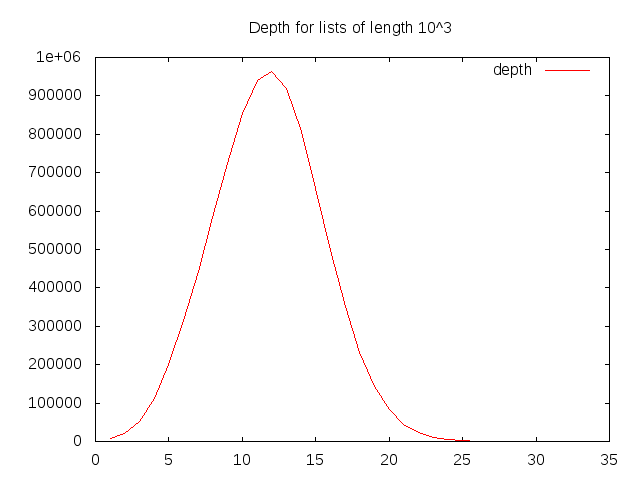
\includegraphics[scale=0.3]{images/3.png}
\end{center}
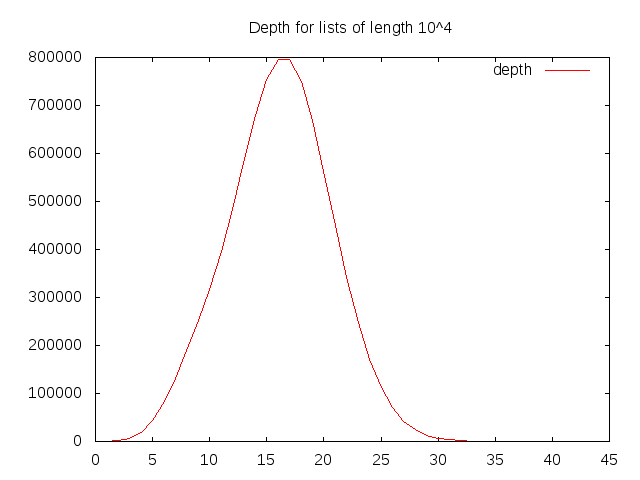
\includegraphics[scale=0.3]{images/4.png}
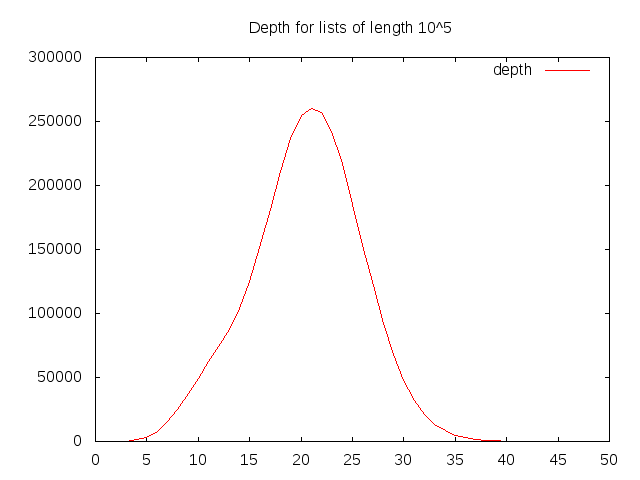
\includegraphics[scale=0.3]{images/5.png}
\subsection*{\texttt{QUICKSORT}}

{\bf 1.7 \ Subproblem} Let $X$ denote the number of comparisons made by
randomized QUICKSORT on an input of length $n$. We know that $E[X]
\leq \mu_s= 2n\ln n$.  Prove that the probability that the number of
comparisons made in an execution of randomized QUICKSORT exceeds
$3\mu_s$ is at most $2n^{-d}$ for as large a constant $d$ as you can.`
Hint: Show that $\Pr(X>3\mu_s)\leq n\cdot\Pr(Z>3\mu)$.

The initial inequality $\Pr(X>3\mu_s)\leq n\cdot\Pr(Z>3\mu)$ can be explained by having an indicator variable

$$X_{ij}=\left\{\begin{array}{ll}
1, & \mbox{
\begin{minipage}[t]{4in}
  if $i$ is selected as a pivot element and if i and j are compared to each other 
\end{minipage}
}
\\
0, & \mbox{ otherwise}
\end{array}\right.$$

We then have $X = \sum_{i \neq j} X_{ij} = \sum_j \left( \sum_{i \neq j} X_{ij} \right)$. We notice that the inner sum, $ \sum_{i \neq j} X_{ij}$, is the amount of pivot elements chosen and can be compared to the amount of pivot elements chosen in \texttt{FIND}. So there is a correlation between $Z$ and $X$. The outer sum, $\sum_j$, translates to a factor $n$ on the inner sum. Each time a pivot element is chosen in \texttt{QUICKSORT} up to $n$ comparisons are made. With this in mind we notice that $\Pr(X>3\mu_s)\leq n\cdot\Pr(Z>3\mu)$ holds because that while $Pr(X > 3\mu_s)$ and $Pr(Z > 3\mu)$ are roughly equal, the added factor $n$ makes the inequality hold. We now compute the upper bound of $Pr(Z > 3\mu)$ and apply it to our \texttt{QUICKSORT}:

\begin{align*}
n\cdot \Pr[Z>3\mu] &\leq n\cdot \left [ \frac{e^2}{3^2} \right ]^{2\ln n}\\
&=n\cdot\frac{e^{4\ln n}}{9^{2\ln n}} =\frac{n^5}{9^{2\ln n}}\\
&=\frac{n^5}{e^{\ln 9 \ln n^2}} =\frac{n^5}{n^{2\ln 9}}\\
&=\frac{n^5}{n^{\ln 9}n^{\ln 9}} =n^{5-2\ln 9}
\end{align*}

We now have an upper bound for half of the quicksort algorithm seeing that it will be split into two recursively. Doubling the upper bound will result in the upper bound for quicksort. With this in mind we have that $Pr(Z > 3\mu)$ is upper bounded by $2n^{5-2\ln(9)}$ and thusly  find that $\underline{d = 2\ln(9) - 5}$.
\par
We have run the same experiments as for the \texttt{FIND} algorithm. The results can be seen in \ref{tab:quicksort}.
As can be seen from the table, the algorithm does not on average exceed our bound, and there is a quite large margin between the average case and the bound on the expected average. We even see as we approach larger n, that our worstcase becomes relatively less larger than our expected average, which is a very nice quality to have.
\begin{center}
\begin{figure}
\caption{Results from running \texttt{QUICKSORT}}
\label{tab:quicksort}
\begin{center}
\begin{tabular}{| c | c | c | c |}
\hline
\emph{n} & Avg. Comp. & Max Comp. & $2nlnn$\\ \hline
$10^2$ & 509 & 1177 & 921.03\\ \hline
$10^3$ & 9280 & 16809 & 13815.51 \\ \hline
$10^4$ & 138868 & 206495 & 184206.81\\ \hline
\end{tabular}
\end{center}	
\end{figure}
\end{center}

{\bf 1.9 \ Implementation}

For our pseudo-random numbers we have used the C++11 implementation of the Mersenne Twister algorithm, the std::mersenne\_twister\_engine. Reference: \url{ http://en.cppreference.com/w/cpp/numeric/random/mersenne_twister_engine}. We are using a uniform\_int\_distribution to find a random number in a given range. 

Our \texttt{FIND} method uses the Standard Library partition\_copy method combined with a lambda expression to partition the list over into two lists with the condition that $i$ is either bigger or smaller than the randomly chosen element $e$.

When generating a random list of integers we first generate a list containing $1,2,\ldots, n-1,n$ elements utilizing generate\_n and a lambda expression and then we randomly shuffle them using the Standard Library shuffle function in conjunction with our mersenne twister engine. This way we make sure we only have unique elements in our list. Seeing as the randomness of this list is not so important because we are randomly choosing an element from it we only regenerate the list once we need one of another size.

\end{document}
